%!TEX root = foo-thesis.tex

\chapter{Uniqueness}
\label{chap:uniqueness}

Die zu klassifizierenden Objekte und deren einzelne Punkte sollten sich - im ein oder anderen Featureraum - merklich unterscheiden von den gewöhnlichen Straßenpunkten, die weder einen Schaden noch ein sonstiges besonderes Objekt darstellen. Dieses Konzept der \textit{uniquen} Punkte, teilweise auch \textit{key feature points}, hat das Ziel eine Punktwolke durch eine geeignete und angemessen große Menge von Punkten zu charakterisieren. \\
Da, wie bereits erläutert, die Features von verschiedenen Objekten teils erst bei verschiedenen Scales Unterscheidungskraft besitzen, gilt dies auch für die letztlich auf diesen Features basierende \textit{Uniqueness}. Daher wird jene pro Scale berechnet und jeder Punkt, der in mindestens einem Scale \textit{unique} ist, ist dies für die gesamte Punktwolke. Damit darüber hinaus bei stark unterschiedlichen Binzahlen der verschiedenen Featureräume - wenn etwa \textit{Curvature} doppelt so viele Bins hätte wie die Intensitätsdifferenzen - kein einzelner Featureraum einen zu starken Einfluss auf die Entscheidung zur \textit{Uniqueness} hat, wird letztere separat für jeden Featureraum berechnet. Sobald ein Punkt in mindestens einem Featureraum als \textit{unique} gilt, tut er dies auch für den gesamten Scale. Dieses Prinzip ist vor allem mit Blick auf potenzielle zukünftige Erweiterungen eingeführt worden, sollten zum Beispiel neue Features hinzukommen oder sich die Kennzahlen der Histogramme deutlich ändern. In der in diesem Ansatz genutzten Konfiguration, in der alle Histogramme dieselbe Größe besitzen, hat es geringe Auswirkungen. \\
Die Basis für die Ermittlung dieser \textit{uniquen} Punkte, wie vom Prinzip her auch in \cite{Rusu.etal-2008} genutzt, sind 
\begin{itemize}
    \item die Berechnung des Featureraums vom \textit{durchschnittlichen} Punkt (\textit{Mean})
    \item die Berechnung der Distanz zwischen dem Featureraum eines einzelnen Punktes und dem \textit{Mean}-Featureraum
\end{itemize}
Der \textit{Mean}-Featureraum kann für einwertige Features durch einfaches Bilden des Durchschnitts ermittelt werden, für mehrwertige Features werden die \textit{Counts} der einzelnen Bins über alle Punkte gleich gewichtet aufsummiert und entsprechend die \textit{Frequencies} neu berechnet. Umgesetzt wird dies durch die \texttt{mean}-Methode der \texttt{Histogram}-Klasse. \\\\
Diejenigen Punkte, die eine spezifizierte ausreichend große Distanz zum \textit{Mean} besitzen, werden anschließend als \textit{unique} betrachtet. Das genutzte Distanzmaß ist dabei die \textit{Kullback-Leibler-Divergenz (KL-Divergenz)} \citep{Kullback.Leibler-1951}. Dieses ist originär ein nicht-kommutatives Maß über zwei Wahrscheinlichkeitsverteilungen $P$ und $Q$ und drückt den Grad ihrer Verschiedenheit aus. In diesem Ansatz werden keine Wahrscheinlichkeitsverteilungen in jenem Sinne verwendet, doch die mehrwertigen Features in Form von Histogrammen erfüllen ihre nötige Eigenschaften: Alle Einträge, in diesem Fall die \textit{Frequencies} der Bins, liegen zwischen 0 und 1 und ihre Gesamtsumme beträgt genau 1. Für einwertige Features ist die zweite Eigenschaft nicht erfüllt, sie machen aber nur einen kleinen Teil der vollständigen Featurevektoren aus und werden aus Gründen der Praktikabilität dennoch identisch behandelt. \cite{Rusu.etal-2008} nutzen die KL-Divergenz ebenfalls als eines von mehreren getesteten Distanzmaßen. \\
$P$ steht hierbei jeweils für den Featureraum eines Punktes, $Q$ für den \textit{Mean}-Featureraum eines Scales. Die Formel zur Berechnung der Distanz zwischen diesen Featureräumen, wobei $P(i)$ und $Q(i)$ die \textit{Frequencies} der jeweils $i$-ten Bins und $n$ die Binzahl bezeichnen, lautet:
\begin{equation}    
    D(P || Q) = \sum_{i=1}^{n}{(P(i) - Q(i)) * \log_2\left(\frac{P(i)}{Q(i)}\right)}
\end{equation}
Die KL-Divergenz ist nur definiert, wenn für alle Einträge $i$ mit $Q(i)=0$ auch $P(i)=0$ gilt. Dies ist hier der Fall, da ein Eintrag von 0 im \textit{Mean} immer bedeutet, dass der entsprechende Eintrag auch beim Featureraum jedes Punktes gleich 0 ist. Für $P(i)=0$ ist der Summand als 0 definiert. \\
Von der Liste all der parallel berechneten Distanzen zum \textit{Mean} werden daraufhin der Durchschnitt $\mu$ sowie die Standardabweichung $\sigma$ ermittelt. Ein Punkt $P$ ist nun genau dann \textit{unique}, wenn gilt:
\begin{equation}
    D(P || Q) \geq \mu + \alpha * \sigma
\end{equation}
Dabei ist $\alpha$ ein im \texttt{PavementDistressDetector}-Knoten einstellbarer Parameter. Je größer dieser ist, desto weniger Punkte gelten tendenziell als \textit{unique} - diese sind dafür aber besonders auffällig. In den Experimenten hat sich generell ein Wert von 1,0 als annehmbar dargestellt. Eine Evaluierung verschiedener $\alpha$-Werte findet sich in Kapitel \ref{chap:eval}. \\\\
Die Gründe für eine solche Darstellung der Punktwolke durch eine geringere Zahl an Punkten sind vielfältig. Eine Motivation kann - gerade für statische Objekte - die Registrierung sein. Dabei sind die Ausgangslage zwei oder mehr Punktwolken, die durch mehrere Laserscannungen entstanden sind, etwa zu verschiedenen Zeitpunkten oder aus unterschiedlichen Perspektiven. Durch geeignete Algorithmen wie dem \textit{Sample Consensus Initial Alignment} \citep{Rusu.etal-2009} können für \textit{unique} Punkte der einen Punktwolke sogenannte Korrespondenz-Punkte in der anderen Punktwolke gesucht werden. Der Vorteil der Nutzung von \textit{Uniqueness} liegt hierbei darin, dass die Ausgangsmenge der zu betrachtenden Punkte für die Korrespondenzsuche drastisch, aber zugleich sinnvoll reduziert wird. Diese tiefgreifendere Verwendung des \textit{Uniqueness}-Konzepts wird in dieser Arbeit nicht näher behandelt, doch in Kapitel \ref{chap:outro} finden sich Ideen für seine Einsatzmöglichkeiten bei der Dokumentation von Straßenschäden. \\
Ein zweiter und pragmatischer Grund für die Ermittlung von \textit{uniquen} Punkten ist die resultierende Datenreduktion. Wie im vorherigen Kapitel erläutert, ist in der momentanen Architektur dieses Ansatzes eine Übertragung der Featurevektoren mit temporärer Festplattenspeicherung nötig. Da weiterhin die Nutzung von mehrwertigen Features wie Histogrammen inhärent zusätzlichen Speicheraufwand bedeutet, soll das \textit{Uniqueness}-Konzept Abhilfe schaffen. Ein weiterer Nebeneffekt ist die reduzierte Trainings- und \textit{Prediction}-Zeit des Modells, da weniger Eingaben zu verarbeiten sind. \\
Eine Bedingung für gute Ergebnisse der \textit{Uniqueness} ist in diesem Anwendungsfall, dass die Objekte von Interesse eine Minderheit der Punkte repräsentieren und so in der Gesamtpunktwolke entsprechend auffallen. Dies ist bei gewöhnlichen Punktwolken von Straßen der Fall, siehe Kapitel \ref{chap:eval} für Relationen der Klassen bei der Trainings- und Testpunktwolke. Für die nicht-\textit{uniquen} Punkte wird die implizite Annahme getroffen, dass diese den gewöhnlichen Straßenzustand repräsentieren, weshalb ihnen direkt die entsprechende Klasse zugewiesen wird. \\\\
Eine visuelle Darstellung des gesamten ersten Teils vom \textit{Feature-Extraction}-Ansatz, der Featureberechnung im \texttt{PavementDistressDetector}-Knoten, findet sich in Abbildung \ref{fig:feature_extraction}. 
Den Abschluss bildet dabei das Schreiben der sogenannten \textit{Featuresdatei}. Diese im Sinne der Speichereffizienz binäre Datei enthält die vollständigen Featurevektoren aller Punkte. Im Falle von betrachteter \textit{Uniqueness} sind nur die Vektoren der \textit{uniquen} Punkte geschrieben inklusive ihrer Indizes. Zusätzlich stehen immer zu Beginn die Gesamtzahl der folgenden Featurevektoren, die Anzahl der genutzten Scales sowie die Featurevektorgröße pro Scale. Die Featuresdatei wird anschließend von den Python-Skripten eingelesen und für Training und Test der Modelle bzw. die abschließende \textit{Prediction} der Klassen genutzt, siehe Kapitel \ref{chap:prediction}.

\begin{figure}[!ht]
    \centering
    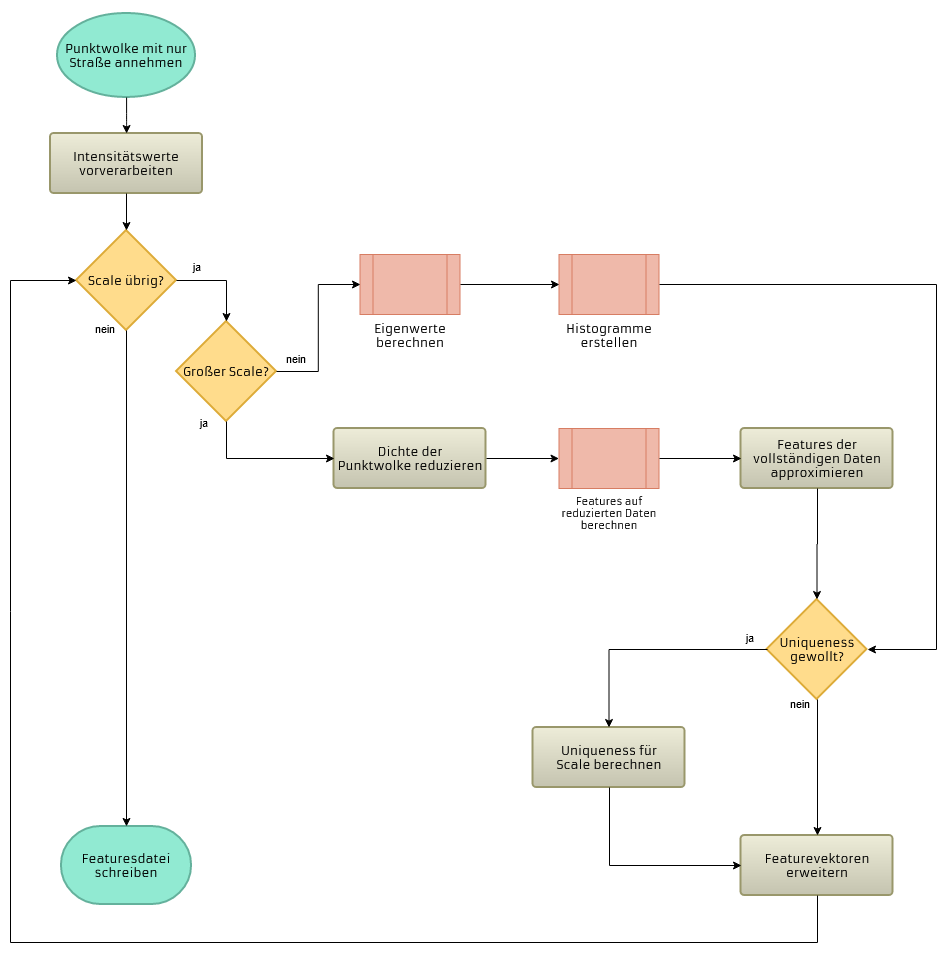
\includegraphics[width=0.98\textwidth]{graphics/flowchart_feature_extraction}
    \caption{Eine Übersicht des Ablaufs der Featureberechnung. Die roten Kästen kennzeichnen die bezüglich Laufzeit aufwändigsten Schritte des Prozesses.}
    \label{fig:feature_extraction}
\end{figure}